A felhasználó felületnek a képekben való bemutatása nehéz, főleg a "Vigyél el" funkció. Ezért van egy demó verzió amelyet jelenleg meglehet tekinteni a következő címen: http://193.226.0.198:20024. 

\section{A 3D modell megjelenése}

Az alkalmazás indításakor elsőre a 3D modell jelenik meg. Ez látható a \ref{fig:modell3D} ábrán. A modellen kívül megjelenik egy legördülő lista, ahol a Visitorok kitudnak választani egy fontos egyetemi helyet és plusz gomb megjelenésével eltudnak navigálni oda. Ez megfigyelhető a \ref{fig:takeMe} ábrán. Látható hogy ki lett választva az Aula és \ref{fig:modell3D} ábrától eltérően megjelent egy újabb gomb egy emberkével. Ez a gomb jelzi az alkalmazásnak, hogy a Visitor elszeretne jutni valahová. Ha ezt a gombot nyomjuk akkor az alkalmazás bemutatja a bejárattól az utat a kiválasztott helyre, esetünkben a bejárattól az Auláig.
\begin{figure}[H]
	\centering
	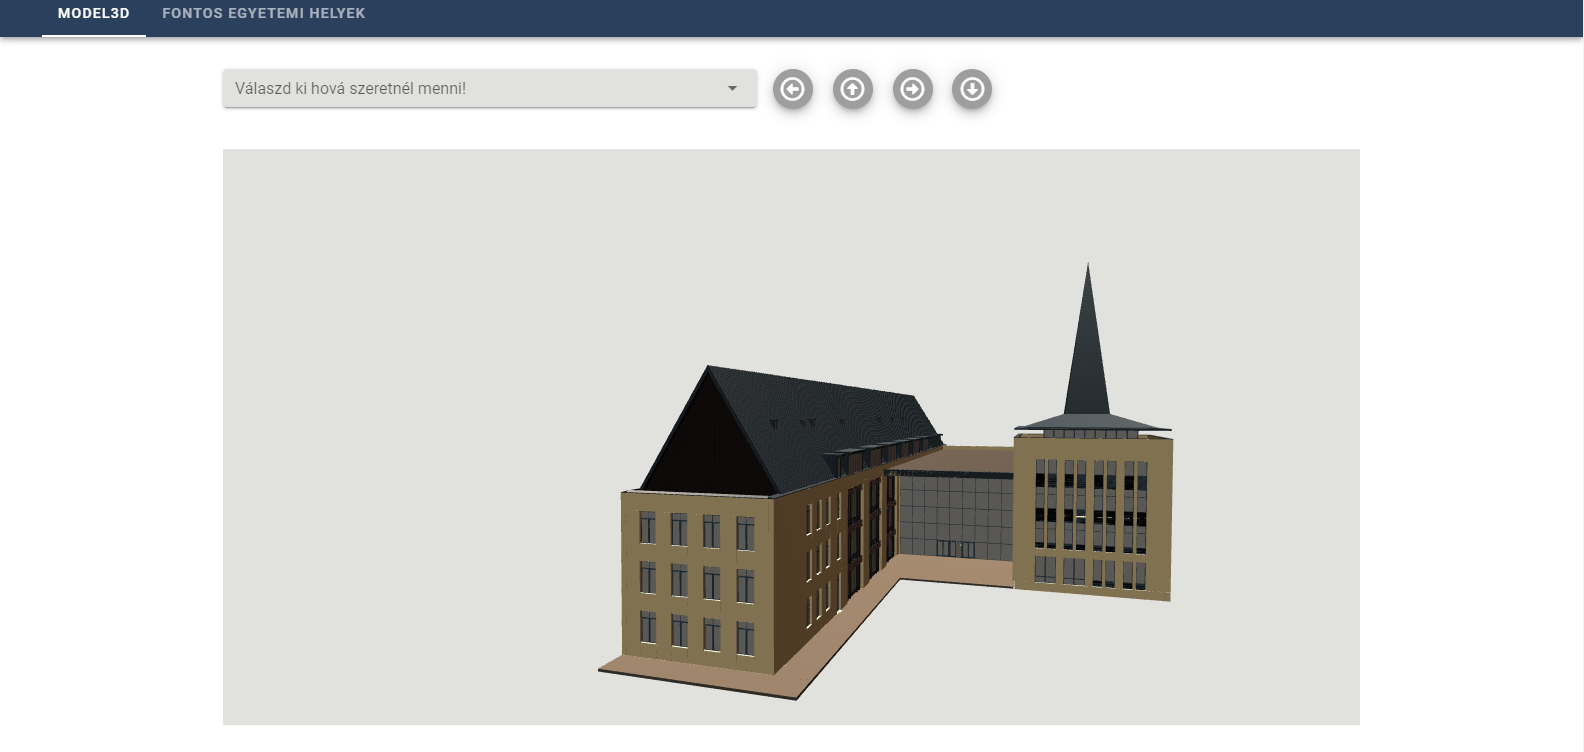
\includegraphics[width=0.9\linewidth]{figures/images/3dmodell.png}
	\caption[3D modell megjelenése az alkalmazásban]{\textit{3D modell megjelenése az alkalmazásban}}
	\label{fig:modell3D}
\end{figure} 

\begin{figure}[H]
	\centering
	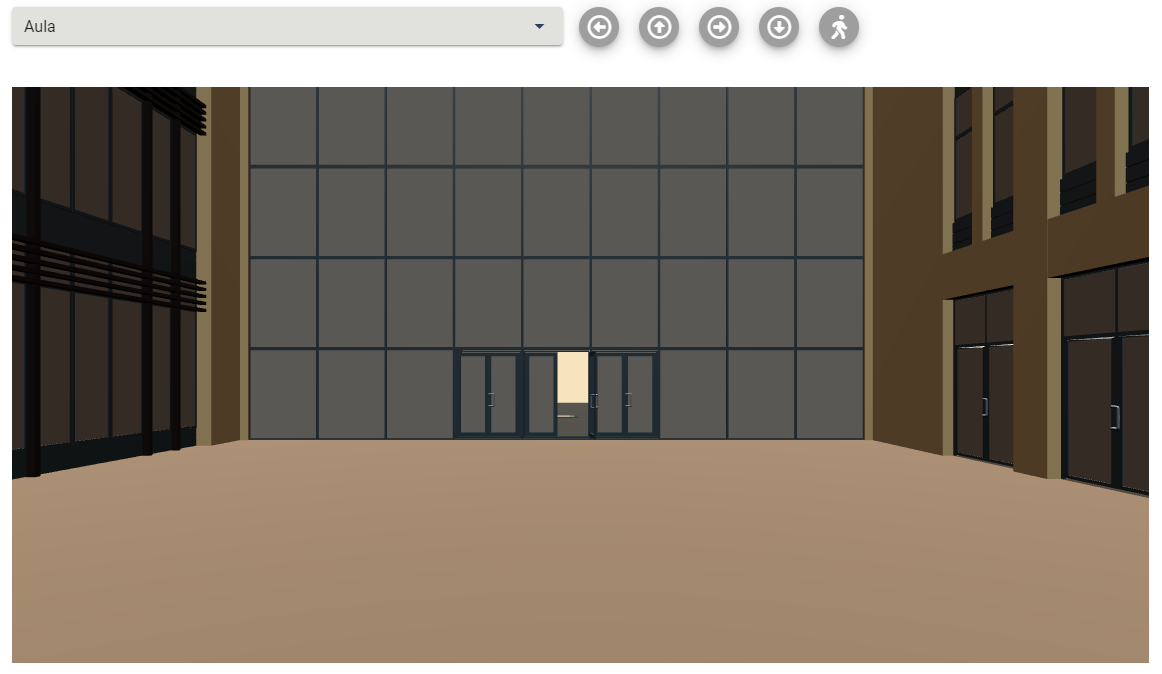
\includegraphics[width=0.9\linewidth]{figures/images/vigyelEl.png}
	\caption["Vigyél el" funkció részleges bemutatása]{\textit{"Vigyél el" funkció részleges bemutatása}}
	\label{fig:takeMe}
\end{figure} 

A \ref{fig:bejartaAula} ábrán látható, hogy az ábrának az első részében még ott vagyunk a bejárat előtt. Ha megnyomjuk a navigálásra alkalmas gombot akkor átkerülünk az ábrának a második részében látható aulába. Ezen kívül az egér segítségével tudunk forogni és a navigációs gomb mellet láthatunk olyan gombokat is amelyeken nyilak vannak. Ezeknek a nyilaknak a segítségével tudunk előre, jobbra, balra és hátra mozogni a modellben. A jobb megértés érdekében érdemes ellátogatni a fent említett címre és kiprobálni a funkciókat.

\begin{figure}[H]
	\centering
	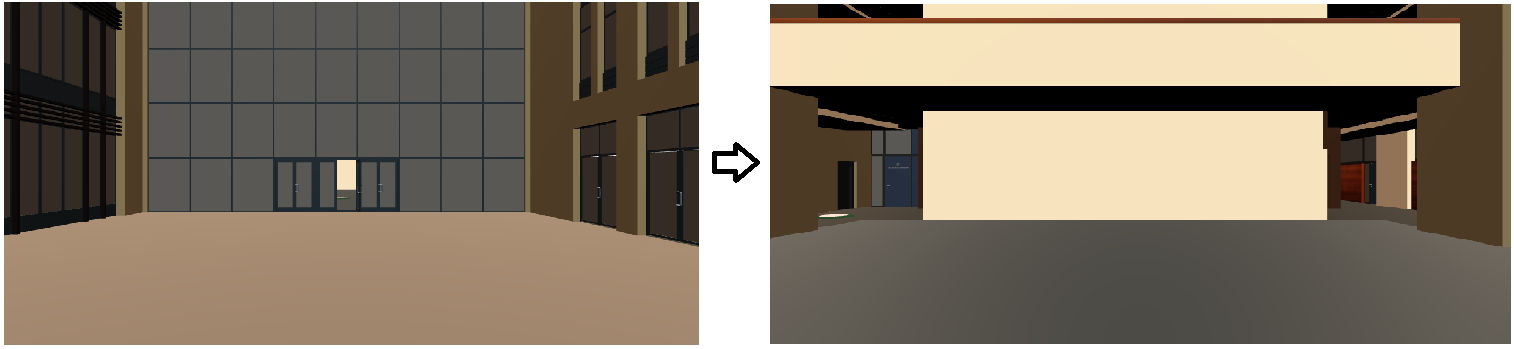
\includegraphics[width=0.9\linewidth]{figures/images/bejaratAula.png}
	\caption[Útvonal megmutatása a bejárattól az Auláig]{\textit{Útvonal megmutatása a bejárattól az Auláig}}
	\label{fig:bejartaAula}
\end{figure} 

\section{Fontos egyetemi helyek megjelenése}

A fontos egyetemi helyeknek a megtekintééhez átkell lépnünk a következő menüpontra. Ha átléptünk a második menüpontra, akkor a \ref{fig:importantPlace} ábrán látható képpel fogunk találkozni. Itt megjelennek a A tanszékek és különböző hivatalok. Ezeken belül megjelennek a különböző alrészlegek vagy egyéb fontos inforációk az adott részleggel kapcsolatban. A címekre kattintva átkerülünk egy másik oldalra ahol, bővebb információkat találunk az adott részlegről. A cím mellett található ikonra kattintva vissza kerülünk a modellhez és az útvonal lesz bemutatva, úgy ahogy az előző részben bemutatódott a bejárat és az Aula között út.

A \ref{fig:vmTan} ábrán bemutatnám miként jelenik meg egy tanszék az alkalmazáson belül. Először is megjelenik a tanszék neve, esetünkben a Villamosmérnöki Tanszék. Ezek után két csoportosítást vehetünk észre. Az alrészlegek tartalmazzák a tanszékhez tartozó szakokat. A jelenlegi ábrán látható az Automatika és alkalmazott informatika, Infokommunikációs hálózatok és rendszerek (Távközlés) és Számítástechnika szakok. A szakok alatt láthatóak információk az adott szakkal kapcsolatban, mint például a szakkoordinátorok neve. Ezek után megjelennek az egyebek kategória, ami az adott tanszékehez tartozó versenyeket (Sapi-Line-Tracer robotverseny), eseményeket írják le. A \ref{fig:utVmTan} ábrán látható egy kép amely bemutatja, hogyan lehet eljutni a Villamosmérnöki tanszékre. A bejárattól kezdődően indulva beérkezünk az aulába, ahonnan tovább haladva elérünk a Gépészmérnöki Tanszék bejáratához. A következő lépésben felmegyünk a lépcsőn és megérkezünk a Titkárság ajtójához. Innen megfordulva és tovább haladva eljutunk a célállomáshoz a Villamosmérnöki Tanszék ajtója elé.

\begin{figure}[H]
	\centering
	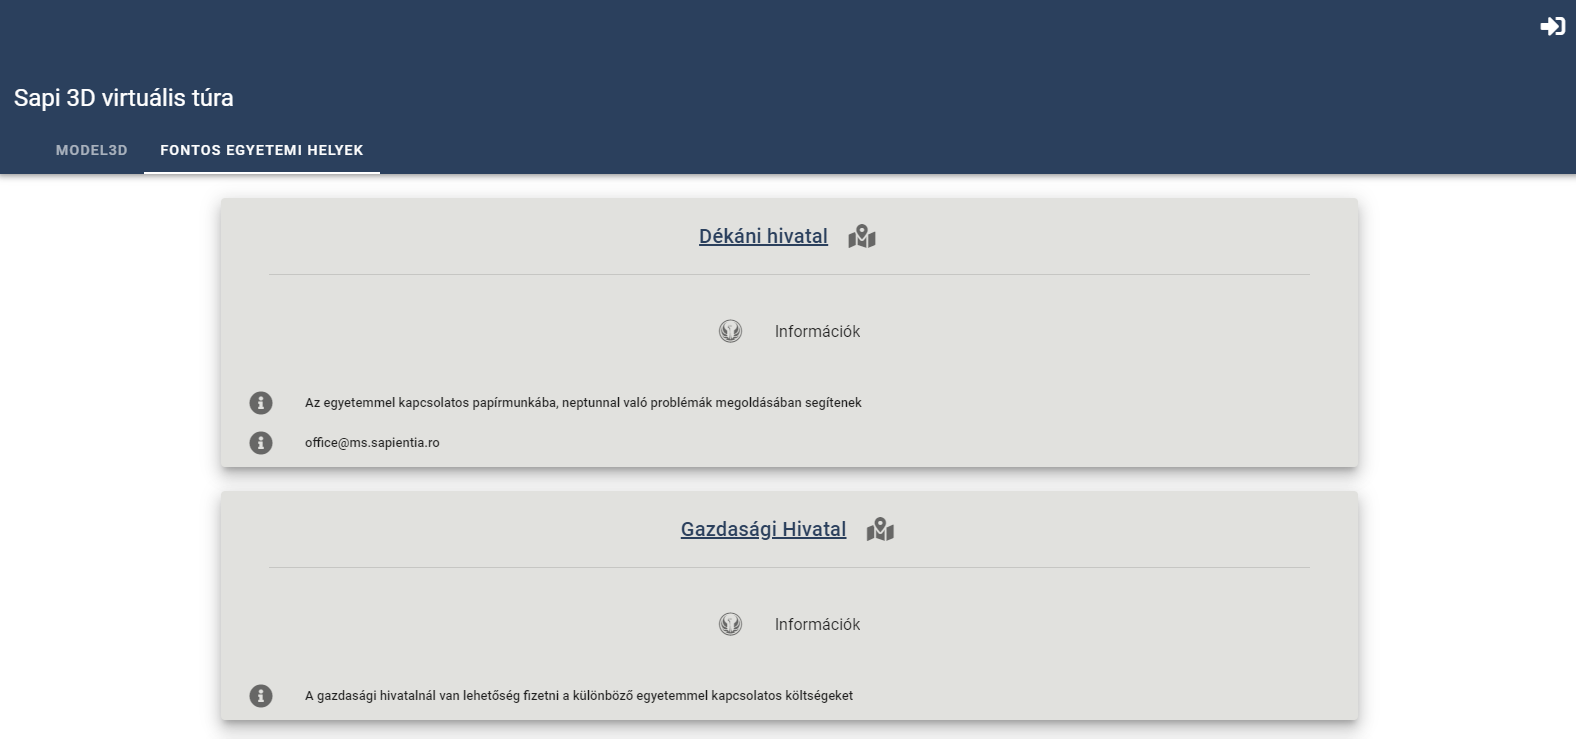
\includegraphics[width=1\linewidth]{figures/images/egyetemiHelyek.png}
	\caption[Fontos egyetemi helyek megjelenése az alkalmazásban]{\textit{Fontos egyetemi helyek megjelenése az alkalmazásban}}
	\label{fig:importantPlace}
\end{figure} 

\begin{figure}[H]
	\centering
	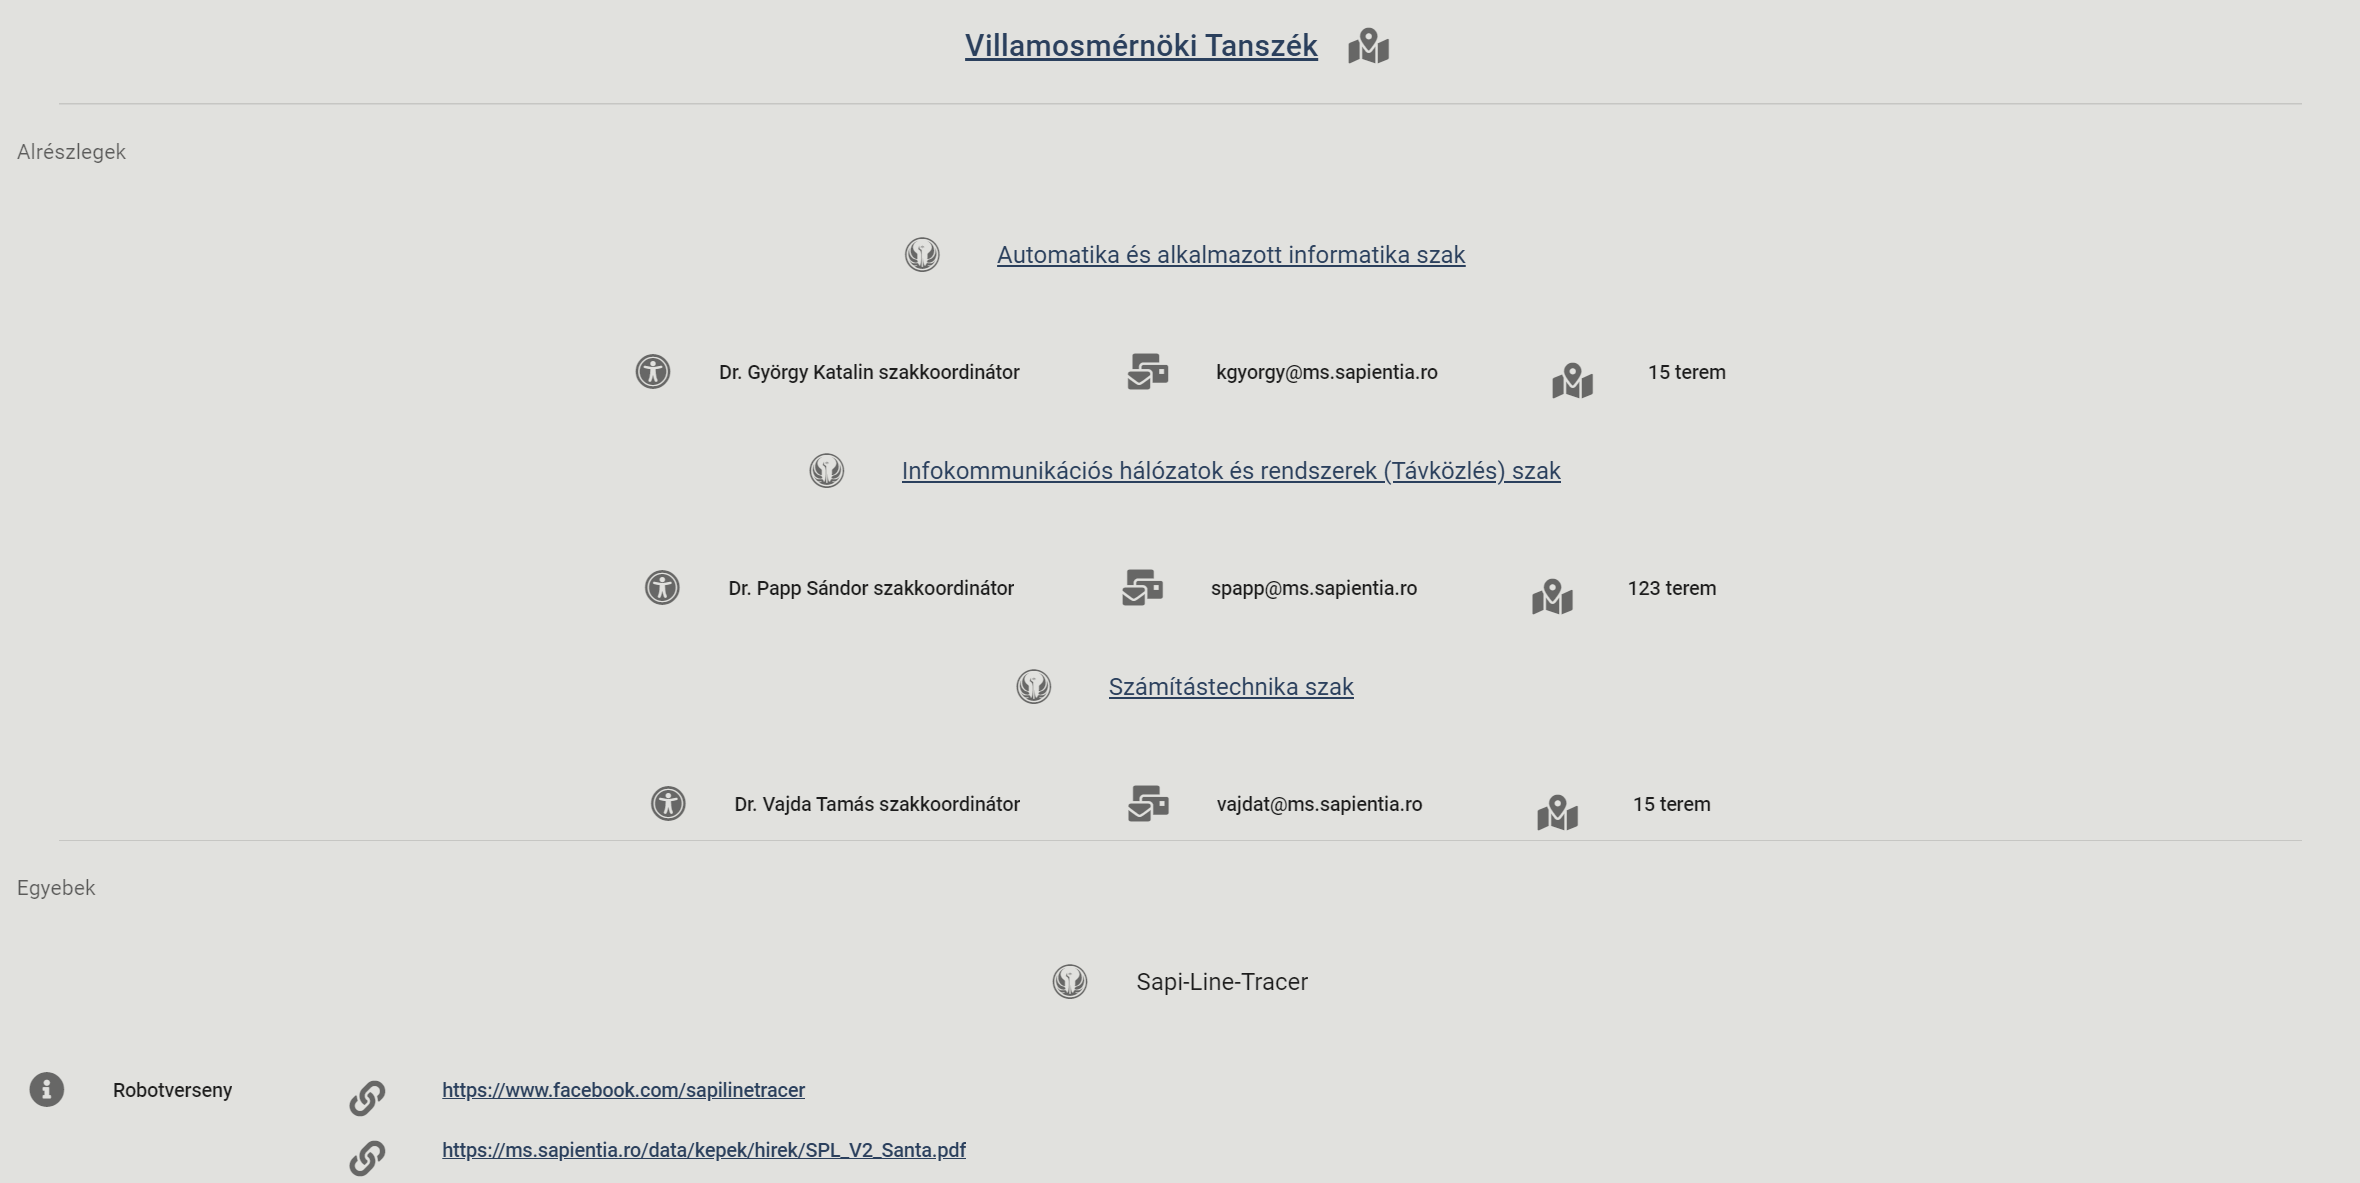
\includegraphics[width=1\linewidth]{figures/images/vmTanMeg.png}
	\caption[Példa a Villamosmérnöki Tanszék megjelenésére]{\textit{Példa a Villamosmérnöki Tanszék megjelenésére}}
	\label{fig:vmTan}
\end{figure} 

\begin{figure}[H]
	\centering
	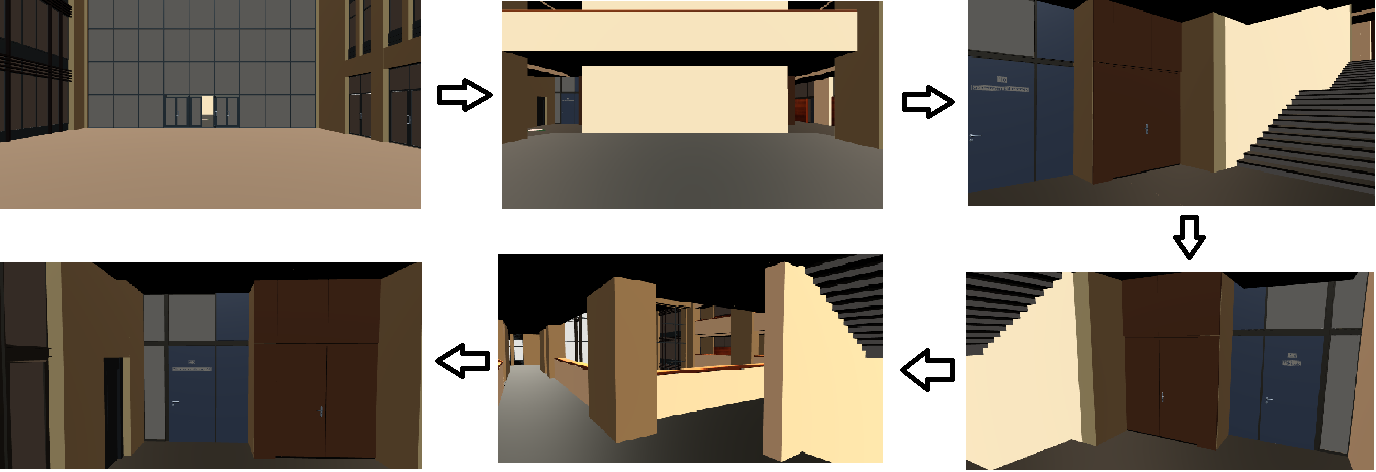
\includegraphics[width=1\linewidth]{figures/images/utVMT.png}
	\caption[Út a Villamosmérnöki Tanszékhez a bejárattól]{\textit{Út a Villamosmérnöki Tanszékhez a bejárattól}}
	\label{fig:utVmTan}
\end{figure} 

\section{Bejelentkezés és kijelentkezés}

A bejelentkezés ablakáról láthatunk képet a \ref{fig:loginWindow} ábrán, ahová a felhasználó betudja írni az e-mail címet és a jelszót. Mindkét mezőt kötelező kitölteni és mindkét mezőbe a megfelőlő formátumot kell írni. Jelszó esetében kis- és nagybetüt valamit számot. A Bejelentkezés gombra kattintva tudunk bejelentkezni, ha megfelelő jelszóval és e-mail címmel rendelkezünk. A jelszót megis tudjuk tekinteni ha rálépünk a label végében található áthúzott szemre. 

A kijelentkezést a weboldal sarkában megjelenő kijelentkező gomb használatával tehetjük meg.
\begin{figure}[H]
	\centering
	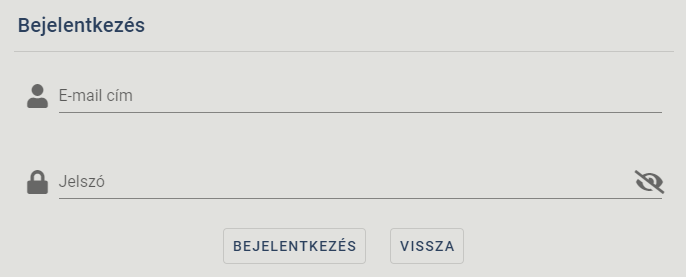
\includegraphics[width=0.7\linewidth]{figures/images/bejelentkezesKep.png}
	\caption[Bejelentkezési ablak megjelenése az alkalmazásban]{\textit{Bejelentkezési ablak megjelenése az alkalmazásban}}
	\label{fig:loginWindow}
\end{figure}

\section{Jelszó hitelesítése}
A jelszó hitelesítésére szolgáló űrlapot a \ref{fig:jelszoHit} ábrán láthatjuk, ahol megjelenik három label, amelyket ki kell kitülteni a tokennel, a jelszóval és a jelszó újrával. A sikeres jelszó megadás akkor lesz, ha a token létezik és a felhasználási idő nincs lejárva. Ezen kívül a két megadott jelszó megkell eggyezzen és kell tartalmazzanak kis- és nagybetűt valamit számot is.
\begin{figure}[H]
	\centering
	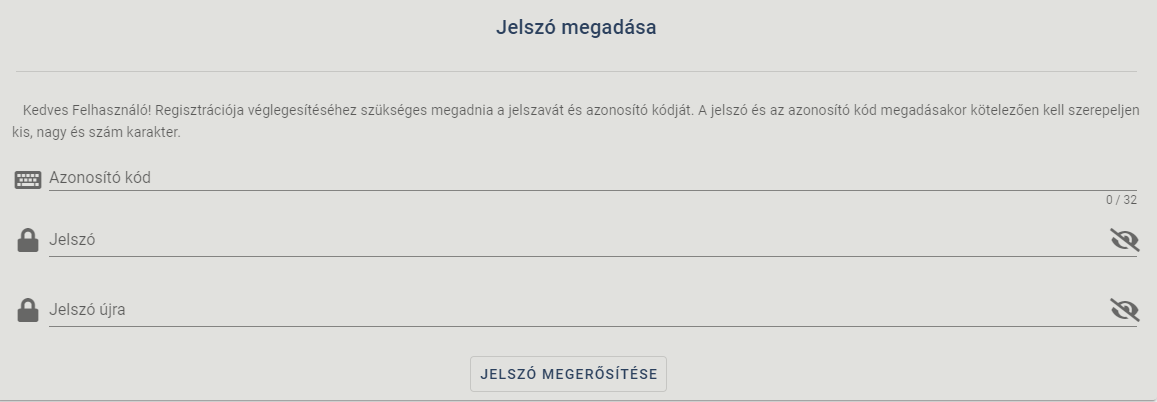
\includegraphics[width=0.7\linewidth]{figures/images/jelszoHit.png}
	\caption[Jelszó hitelesítésére szolgáló űrlap]{\textit{Jelszó hitelesítésére szolgáló űrlap}}
	\label{fig:jelszoHit}
\end{figure}

\section{User adatainak szerkesztése}
A Usernek a bejelentkezés után lehetősége van a saját adatainak a szerkesztésére. A bejelentkezés után a weboldal jobb sarkában megjelenik egy ember ikon, amelyre ha rákattint előjönnek az adatai és a szerkesztési lehetőség, lásd a \ref{fig:userUpdate} ábrán. A szerkesztés esetén egy sort sem lehet üresen hagyni, különben a szerkesztés gomb nem fog működni. 
\begin{figure}[H]
	\centering
	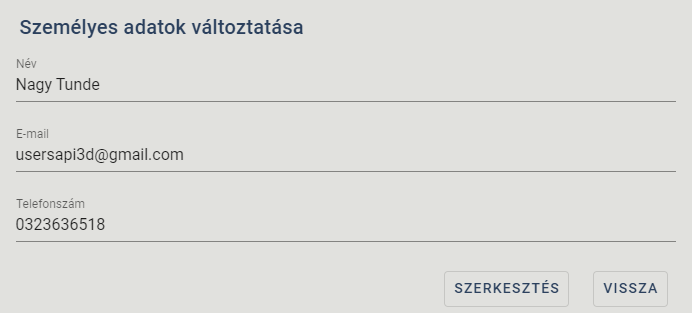
\includegraphics[width=0.7\linewidth]{figures/images/userUpdate.png}
	\caption[User adatak szerkesztésére használható rész]{\textit{User adatak szerkesztésére használható rész}}
	\label{fig:userUpdate}
\end{figure}

\section{User regisztrálása és törlése}
A User regisztrálását és törlését az Admin végzi. \ref{fig:addUser} ábrán látható egy űrlap, amellyel az új User adatait tudjuk regisztrálni. Be kell írni a User nevét, a telefonszámát és az e-mail címét. A Hozzáadás gomb megnyomásával adjuk, hozzá a Usert. Attól függően, hogy a hozzáadás sikeres volt vagy nem a gomb alatt megfog jelenni egy üzenet. 

A User törlésére is szintén egy űrlapot kell használni, amely a \ref{fig:deleteUser} ábrán látható. Első sorban megjeleni egy legördülő list a Userek e-mail címével. Innen kiválasztva a megfelelő e-mail címet lekérjük a User adatatit. Majd ha az adatok alapján a megfelelő személyt választottuk ki, akkor TÖRLÉS gom lenyomásával kitöröljük a Usert.
\begin{figure}[H]
	\centering
	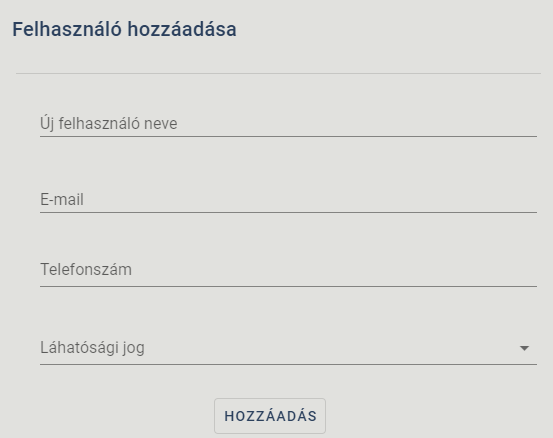
\includegraphics[width=0.7\linewidth]{figures/images/userHozzaadas.png}
	\caption[User regisztrálására használható rész]{\textit{User regisztrálására használható rész}}
	\label{fig:addUser}
\end{figure}

\begin{figure}[H]
	\centering
	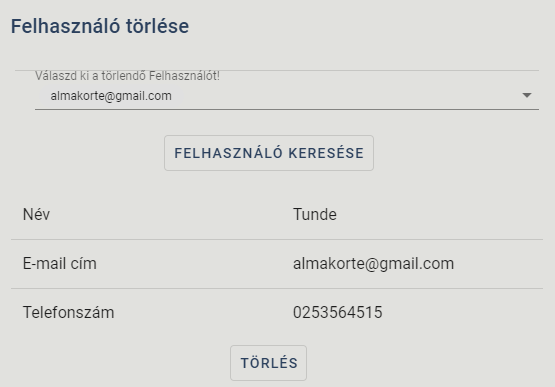
\includegraphics[width=0.7\linewidth]{figures/images/userTorlese.png}
	\caption[User törlésére használható rész]{\textit{User törlésére használható rész}}
	\label{fig:deleteUser}
\end{figure}

\section{Részlegek megadása és szerkesztése}

A részlegek megadása és szerkesztése is egy egy űrlap segítségével történik. A részlegek megadását a \ref{fig:addDepartmentUI} ábrán láthatjuk, ahol látszik, hogy megkell adni egy nevet és egy linket, ahol több információt tudunk elérni az adott részlegről, lásd a \ref{fig:updateDepartmentUI}. Itt az első lépés a részleg kiválasztása, majd amiútán megjelentek a részleg részletei lehet őket szerkeszteni és a szerkesztés gomb megnyomásával véglegesítődik a szerkesztés.
\begin{figure}[H]
	\centering
	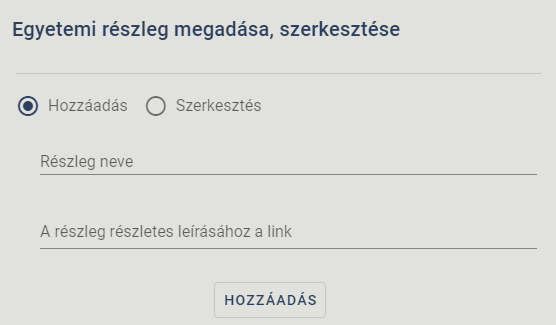
\includegraphics[width=0.7\linewidth]{figures/images/reszlegHozzaadas.png}
	\caption[Részleg hozzáadására alkalamas űrlap]{\textit{Részleg hozzáadására alkalamas űrlap}}
	\label{fig:addDepartmentUI}
\end{figure}

\begin{figure}[H]
	\centering
	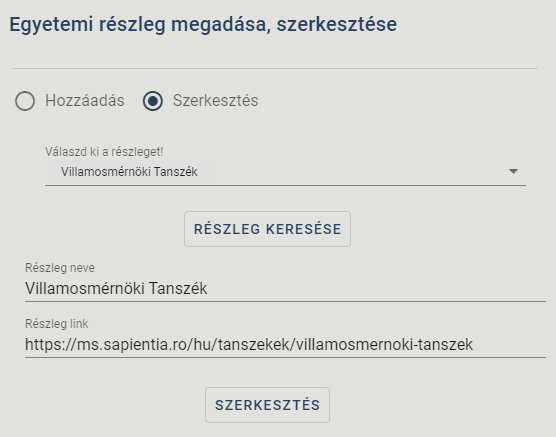
\includegraphics[width=0.7\linewidth]{figures/images/reszlegSzerkesztese.png}
	\caption[Részleg szerkesztésére alkalamas űrlap]{\textit{Részleg szerkesztésére alkalamas űrlap}}
	\label{fig:updateDepartmentUI}
\end{figure}

\section{Szakok megadása és szerkesztése}
A szakok megadása és szerkesztése hasonlóan működik, mint a részlegek megadása és szerkesztése. Az erre alkalmas űrlapokat a \ref{fig:addBranch} és a \ref{fig:updateBranch} ábrákon láthatóak.
\begin{figure}[H]
	\centering
	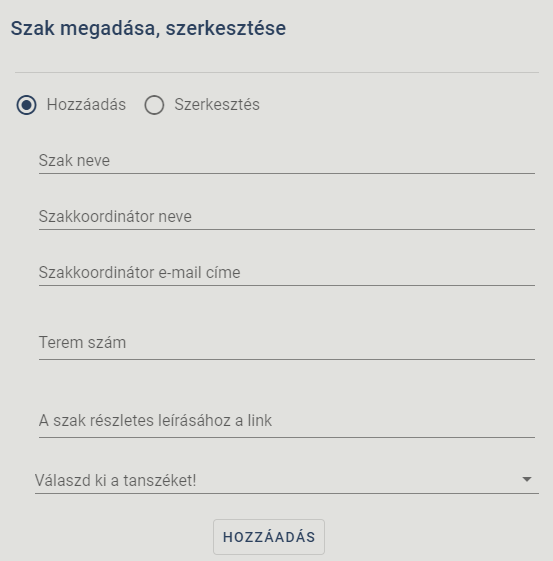
\includegraphics[width=0.7\linewidth]{figures/images/szakMegadasa.png}
	\caption[Szak hozzáadására alkalamas űrlap]{\textit{Részleg hozzáadására alkalamas űrlap}}
	\label{fig:addBranch}
\end{figure}

\begin{figure}[H]
	\centering
	\includegraphics[width=0.7\linewidth]{figures/images/szakSzerkesztése.png}
	\caption[Szak szerkesztésére alkalamas űrlap]{\textit{Részleg szerkesztésére alkalamas űrlap}}
	\label{fig:updateBranch}
\end{figure}

\section{Egyebek megadása}
Az egyebek megadására az űrlap a \ref{fig:addOtherBranch} ábrán látható, ahol kikell választani egy részleget, majd lehet hozzáadni szövegrészeket, linkeket. A szövegrészekhez szükséges labelt az űrlap alján található billentyűzet ikonra való kattintással végezhetjük el. A mellette található ikonnal tudjuk a linkek hozzáadását elvégezni. Egy ilyen egyéb kategória megadásánál legalább ki kell tölteni egy szöveges labelt és egy linket tartalmazó labelt is.
\begin{figure}[H]
	\centering
	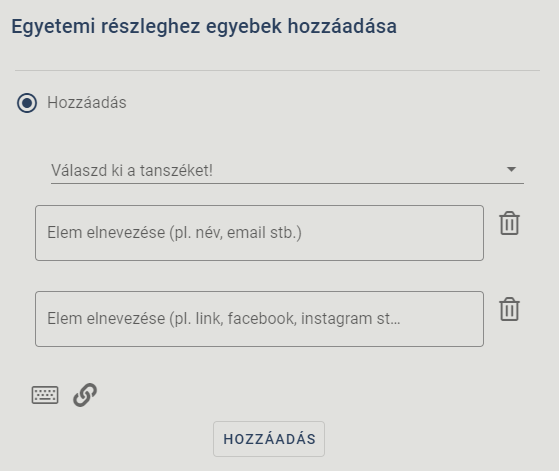
\includegraphics[width=0.7\linewidth]{figures/images/egyebekHozzadasa.png}
	\caption[Egyebek hozzáadására alkalamas űrlap]{\textit{Egyebek hozzáadására alkalamas űrlap}}
	\label{fig:addOtherBranch}
\end{figure}